% TODO: Irgendwo muss beschrieben sein, was genau in meiner Arbeit Echtzeitvisualisierung bedeutet? -> Interpolated schedules. Eventuell könnte dieses Ergebnis auch am Ende von diesem Kapitel erscheinen.

% An open problem is the visualization of real-time vehicles data. The problem relies on the fact that most of todays transit APIs will update bus positions about every minute, and therefore some interpolation is needed to animate vehicles on a map. A very rough approach is to update bus position only when there is a new update, but this cause the vehicle to jump from the old position to the new position and makes it difficult to estimate vehicles movement directions; moreover, the vehicle position is out of date until a new update comes. Although a higher frequency for position updates seems desirable it would also increase the battery consumption on your mobile phone querying the requests while also increase the server load that needs to process it. New visualizations should study how to effectively interpolate bus updates, which is not an easy to solve problem. 
  % [see transit_state_of_the_art.pdf P. 8 section 6.4]

\begin{newpage}
  
  \section{Probleme}
  \label{sec:probleme}

    Die Visualisierung von Echtzeitdaten birgt einige Schwierigkeiten. Nachfolgend sollen mehrere Ansätze auf ihre Vor- und Nachteile für die verwendung auf einer Live-Karte untersucht werden.

    \subsection{Einsatz von GPS Daten}
    \label{sub:einsatz_von_gps_daten}

      \begin{itemize}
        \item \textbf{Fehlende Datenverfügbarkeit:}
          Ein Weg um Echtzeitdaten zu visualisieren, wäre das verarbeiten von GPS Daten. Diese müssten dabei von den jeweiligen Verkehrsverbünden zur Verfügung gestellt werden, was allerdings nicht der Fall ist. Zwar gibt es durchaus eine Erfassung der öffentlichen Verkehrsmitteln, allerdings werden diese nicht für Dritte zur Verfügung gestellt. Die HaCon GmbH sammelt beispielsweise solche Daten, in dem sie diese durch in den Fahrzeug integrierte Software berechnet.\parencite{havasBusradar}. Es wären also GPS Daten vorhanden, da sie unter anderem im Bus-Radar der Deutschen Bahn (entwickelt von HaCon) verwendet werden, sie sind allerdings weder über eine API noch anderweitig für die Öffentlichkeit erhältlich. Über die Rechtlichen belange (dürften in Deutschland solche Daten überhaupt öffentlich gemacht werden), soll an dieser Stelle nicht Diskutiert werden\footnote{In \textit{"`Opening Public Transit Data in Germany"'} von Stefan Kaufmann\parencite{kaufmann} wird dieses Thema der Rechtslage näher betrachtet.}.

        \item \textbf{Aktualisierungsintervall:}
          Abseits der fehlenden Beschaffung von GPS Daten haben diese noch einen weiteren Nachteil. Vehicle die mit einer GPS Lokalisierung ausgestattet sind senden nicht einen kontinuierlichen Strom an Daten, sondern nur in einem gewissen Aktualisierungsintervall. Zwar preist HaCon seinen Busradar durch folgende Aussage an: 

          \begin{quote}
            \textit{"`Der neue Busradar eignet sich hervorragend, um die eigene Fahrt zu visualisieren und Anschlussfahrzeuge zu verfolgen. Erstmals geschieht dies GPS-basiert und nicht durch interpolierte Echtzeitdaten, was eine noch höhere Genauigkeit zur Folge hat."'}\parencite{havasBusradar}
          \end{quote}

          Nimmt man aber nur die GPS Daten als Basis für eine Visualisierung, so springt der Bus immer bei einer Aktualisierung von der jeweilig vorherigen Position zur nächsten. Dieses "`Springen"' kann beim Busradar dann auch dazu führen, dass der Nutzer einen Bus auf seiner App verfolgen will, aber dieser nach dem nächsten GPS Update nicht mehr auf dem Display zu sehen ist, da er nun außerhalb des Viewports liegt. Dieses Verhalten kann den Nutzer durchaus verwirren, da man nicht weiß, in welche Richtung das Vehicle sich bewegt hat und dadurch in alle Richtung gesucht werden muss.

        \item \textbf{Verlässlichkeit \& Verfügbarkeit:} 
          Zudem sind GPS Signale nicht immer verlässlich. Sie können oftmals gestört werden oder die Verbindung zum Satelliten verlieren. Wie würde in einem solchen Fall eines Signalverlusts die Live Visualisierung sich verhalten? Verschwindet das Vehicle von der Karte oder bleibt es für längere Zeit auf der Stelle stehen? Beide Möglichkeiten erscheinen als nicht optimal. 

          Zuletzt sei erwähnt, dass ein GPS basiertes System für U- und S-Bahn erst gar nicht in frage käme, da diese Unterirdisch verlaufen und andere Technologien für deren Erfassung eingesetzt werden müssen. Für eine Live Karte die nicht nur Busse, sondern auch andere Verkehrsmittel abbilden möchte, ist die GPS basierte Lokalisierung folglich nicht zielführend.
      \end{itemize} 

    % subsection einsatz_von_gps_daten (end)

      \subsection{Interpolation von statischen Fahrplandaten}
      \label{sub:interpolation_von_statischen_fahrplandaten}
        In dieser Arbeit wird die Interpolation der statischen Fahrplandaten für die Erstellung der Animation verwendet. Grundlage dafür ist ein GTFS-Feed des Verkehrsverbundes Stuttgart-VVS.
        In diesem Abschnitt sollen die Vor- und Nachteile von einer solchen  Fahrplan Interpolation diskutiert werden.\\

        Ein Nachteil besteht vor allem in einer fehlenden Echtzeitkomponente. Die Fahrplandaten stellen nur einen \texttt{Soll-Zustand} dar, der erheblich vom \texttt{Ist-Zustand} abweichen kann. Auch die Geschwindigkeit eines Vehicles entspricht bei einer Interpolation der Durchschnittsgeschwindigkeit, die sich Anhang der Fahrplandaten ausrechnen lassen. Benötigt ein Vehicle $V$ von Station A nach B 3 Minuten für eine Strecke von 1.2 Kilometer, so würde die Animation eine durchschnittliche Geschwindigkeit von $v = \frac{s}{t} = \frac{1.2 \: \cdot \: 1000}{3 \: \cdot \: 60} = 6.6 \: \frac{m}{s} = 23.76 \: \frac{km}{h}$ errechnen.

        Eine genauere Erfassung der Geschwindigkeit wäre zwar Wünschenswert, bringt allerdings andere Schwierigkeiten mit sich. Die Erfassung der Geschwindigkeit von jedem Vehicle würde eine enorme Menge an Daten bedeuten, die zwischen Server und Client ausgetauscht werden müssen. Ähnlich wie bei einer GPS basierten Animation, wäre der Client komplett davon abhängig, ständig Daten auszutauschen. Stelle man sich vor das mehrere hundert Anwender eine App benutzen wäre dies eine enorme Menge an Anfragen \& Antworten. Für Smartphones mit schlechter Verbindung ist dieser Umstand ein großes Problem. Ebenso wie die verwendete Bandbreite und der erhöhte Batterieverbrauch durch das ständige Stellen von Anfragen und der Verarbeitung der Antwort.

        Die Vorteile ergibt sich aus den eben genannten Nachteilen. Bei einer Interpolation des Fahrplans, ist keine ständige Verbindung zum Server nötig. Existiert der relevante Teil des Fahrplans auf dem Gerät des Endnutzers, so kann die Animation anhand dieser Daten erfolgen. Zudem wird das Problem des "`springens"' Umgangen, welches vor allem bei GPS basierter Animation ein Problem darstellt. Durch die Interpolation sind glatte Animationen der Vehicle auf der Karte möglich. Dies erhöht die User Experience, da der Anwender nachvollziehen kann, wie sich ein Vehicle von A nach B bewegt.
        Eine Lösung für das Problem der fehlenden Echtzeiterfassung ließe sich GTFS-Realtime einsetzen.
      
      % subsection interpolation_von_statischen_fahrplandaten (end)
      
      \subsection{GTFS-Realtime}
      \label{sub:gtfs_realtime}
        Eine andere Möglichkeit für die Erfassung von Echtzeitpositionen und Verspätungen bietet GPS-realtime. GTFS-realtime ist ein von Google entwickelter Standard, der Verkehrsunternehmen das Bereitstellen von Echtzeitinformationen ermöglicht. Dabei gibt es 3 verschiedene Feeds die GTFS-realtime zur Verfügung stellt:\parencite{zervaas_realtime}[S. 6]

        1. Vehicle positions\\
        2. Trip updates\\
        3. Service alerts\\

        GTFS-realtime wäre für diese Arbeit deshalb Interessant, da diese Spezifikation Trip Updates und Vehicle-Position Updates ermöglicht. Beispielsweise kann die Interpolation anhand der Verspätung eines Vehicles angepasst werden. Ein Auszug eines Trip Updates ist in Listing~\ref{lst:gtfs_rt_trip_update} zu sehen.

        \begin{lstlisting}[captionpos=b, caption={Auszug eines GTFS-realtime Trip Updates von MBTA},label={lst:gtfs_rt_trip_update}]
{
  id: 25732950
  trip_update {
    trip {
      trip_id: 25732950,
      start_date: 20150120,
    }
    stop_time_update {
      arival {
        delay: 240
      }
      stop_id: 135
      ...
    }
    ...
  }
}
      \end{lstlisting}

      Vehicle-Positionen können über ein ähnliches Format bezogen werden Listing~\ref{lst:gtfs_rt_vehicle_position_update}.

      \begin{lstlisting}[captionpos={b},caption={Auszug eines GTFS-realtime Vehicle-Position Updates von MBTA},label={lst:gtfs_rt_vehicle_position_update}]
{
  id: "v121",
  vehicle {
    trip {
      trip_id: 2590683,
      start_date: 2017017
    },
    position {
      latitude: 42.267967,
      longitude: -71.093834
    },
    ...
  }
}
      \end{lstlisting}

      In dieser Arbeit kann GTFS-realtime allerdings nicht zum Einsatz kommen, da zum jetzigen Stand, der Verkehrsverbund Stuttgart-VVS dies nicht (auch nicht durch ein anderes Format) öffentlich anbietet. Da GTFS-realtime nicht zur Verwendung kommt, wurde es hier nur ganz kurz und grob beschrieben. Für eine ausführlichere Beschreibung hilft das Buch: \textit{"`The Definitive Guide to GTFS-realtime - How to consume and produce real-time public transportation data with the GTFS-rt specification."'}\parencite{zervaas_realtime} von Quentin Zervaas.\\

      % subsection gtfs_realtime (end)

    \subsection{Bewältigung der Datenmenge}
    \label{sub:bewältigung_der_datenmenge}
      Schon zu Beginn war klar, dass die Anzahl an zu verarbeitenden Daten sehr hoch sein wird. An einem Montag den 28.08.2017 zwischen 3.00 und 24.00 Uhr zeigt Abbildung \ref{fig:activeTrips}: Nach einem rapiden Anstieg in der Morgenzeit, erreicht die Anzahl an aktiven Trips ihre Maxima um 07.04 mit 779. Mittags flacht die Anzahl leicht ab um dann zur Rush Hour am Abend wieder auf 767 Trips anzusteigen. Danach gehen nur noch wenige Trips aktiv. Insgesamt betrug an diesem Tag die Anzahl an absolvierten Trips 19646. In einer Minute gingen maximal 27 und minimal 0 Vehicle aktiv. Im Schnitt starten 9 Vehicles pro Minute ihre Fahrt. 

      \begin{figure}[htbp]
        \begin{center}
          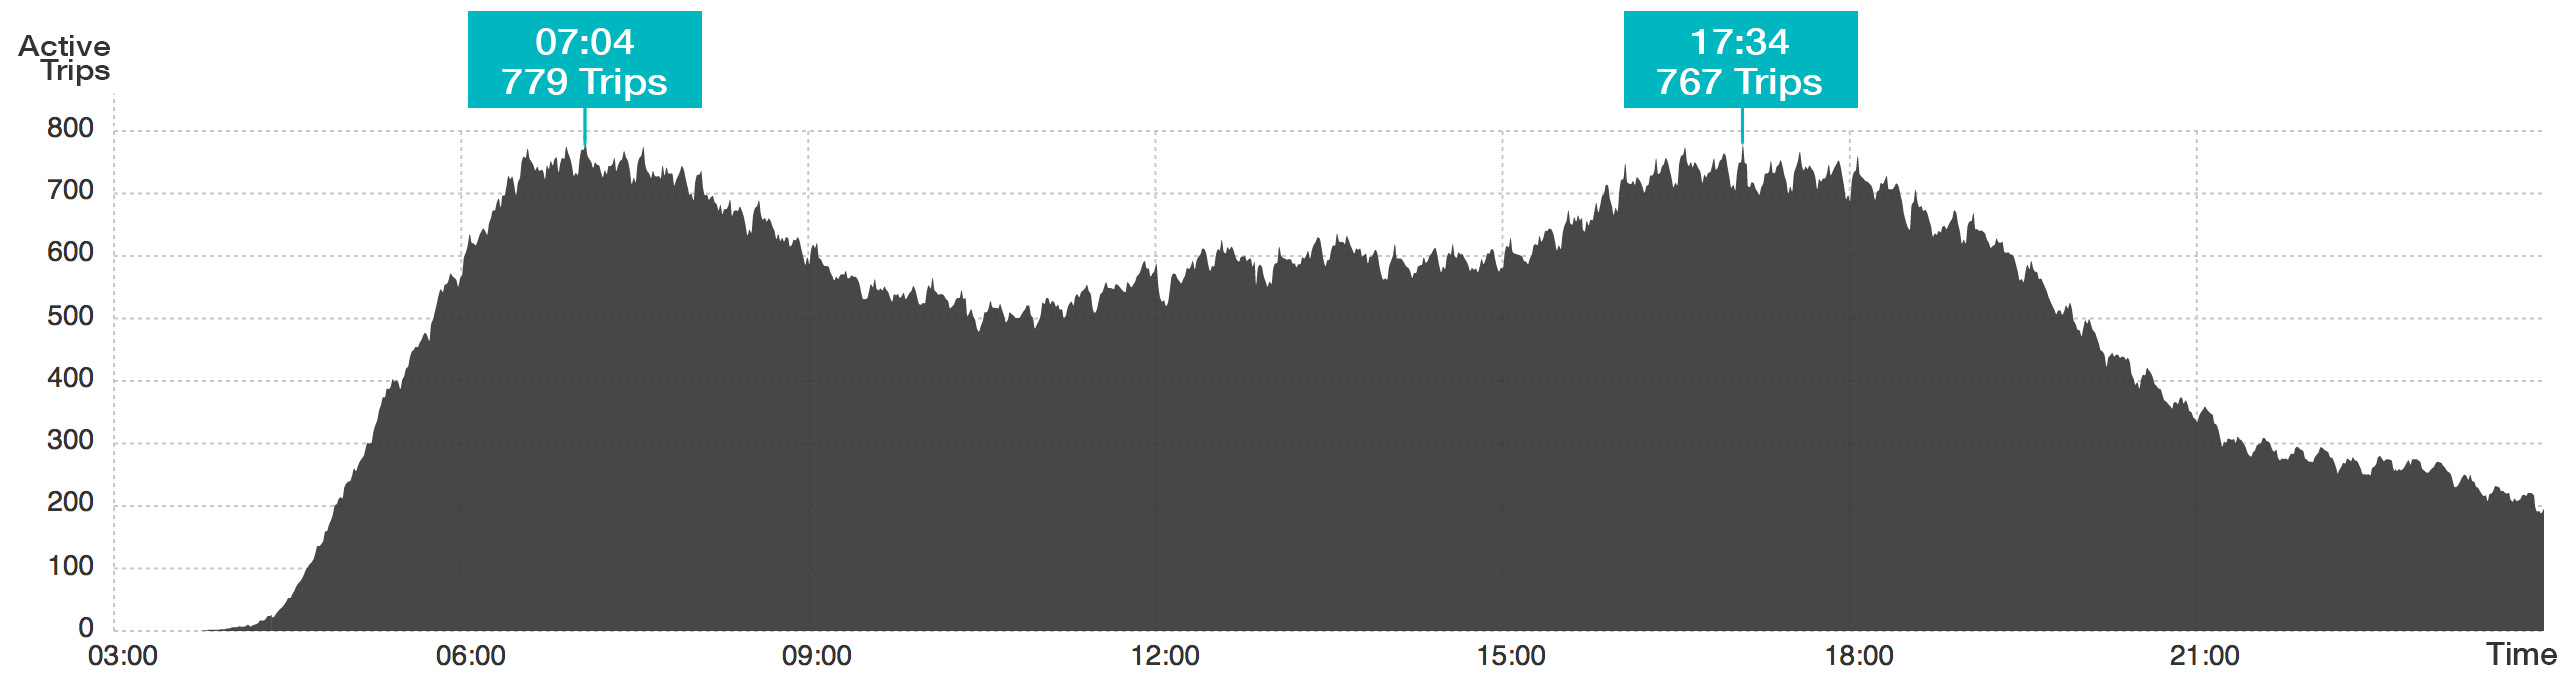
\includegraphics[width=\textwidth]{activeTrips.jpg}
          \caption{Anzahl an aktiven Trips zwischen 3.00 und 24.00 Uhr am 02.08.2017}
          \label{fig:activeTrips}
        \end{center}
      \end{figure}

      Für eine interaktive Karte bedeutet dies, dass je nach Tag zwischen 0 und 1000 Trips aktiv sein können. Dies entspricht dann auch der Anzahl an Vehicles die sie auf der Karte bewegen und animiert werden müssen. Damit dies möglich ist wurde nach Software Lösungen gesucht, die für solche Datenmassen ausgelegt sind. Für die Karte wird dafür Mapbox eingesetzt. Mapbox verwendet Web-GL (basierend auf OpenGL) und bietet damit die Möglichkeit ein GPU unterstütztes Rendering im Browser zu ermöglichen.\\

      Die Wahl der richtigen Tools ist dabei nur die Grundlage um die Datenmenge zu bewältigenden. Viele weitere Schritte sind notwendig um eine performante Webanwendung zu erstellen. Diese werden in Kapitel \ref{sub:backend} \nameref{sub:backend} und \ref{sub:frontend} \nameref{sub:frontend} ausführlich behandelt.
        
    % subsection bewältigung_der_datenmenge (end)
\end{newpage}